%%=============================================================================
%% Methodologie
%%=============================================================================

\chapter{\IfLanguageName{dutch}{Methodologie}{Methodology}}%
\label{ch:methodologie}

%% TODO: In dit hoofstuk geef je een korte toelichting over hoe je te werk bent
%% gegaan. Verdeel je onderzoek in grote fasen, en licht in elke fase toe wat
%% de doelstelling was, welke deliverables daar uit gekomen zijn, en welke
%% onderzoeksmethoden je daarbij toegepast hebt. Verantwoord waarom je
%% op deze manier te werk gegaan bent.
%% 
%% Voorbeelden van zulke fasen zijn: literatuurstudie, opstellen van een
%% requirements-analyse, opstellen long-list (bij vergelijkende studie),
%% selectie van geschikte tools (bij vergelijkende studie, "short-list"),
%% opzetten testopstelling/PoC, uitvoeren testen en verzamelen
%% van resultaten, analyse van resultaten, ...
%%
%% !!!!! LET OP !!!!!
%%
%% Het is uitdrukkelijk NIET de bedoeling dat je het grootste deel van de corpus
%% van je bachelorproef in dit hoofstuk verwerkt! Dit hoofdstuk is eerder een
%% kort overzicht van je plan van aanpak.
%%
%% Maak voor elke fase (behalve het literatuuronderzoek) een NIEUW HOOFDSTUK aan
%% en geef het een gepaste titel.
\begin{figure}[h]
    \centering
    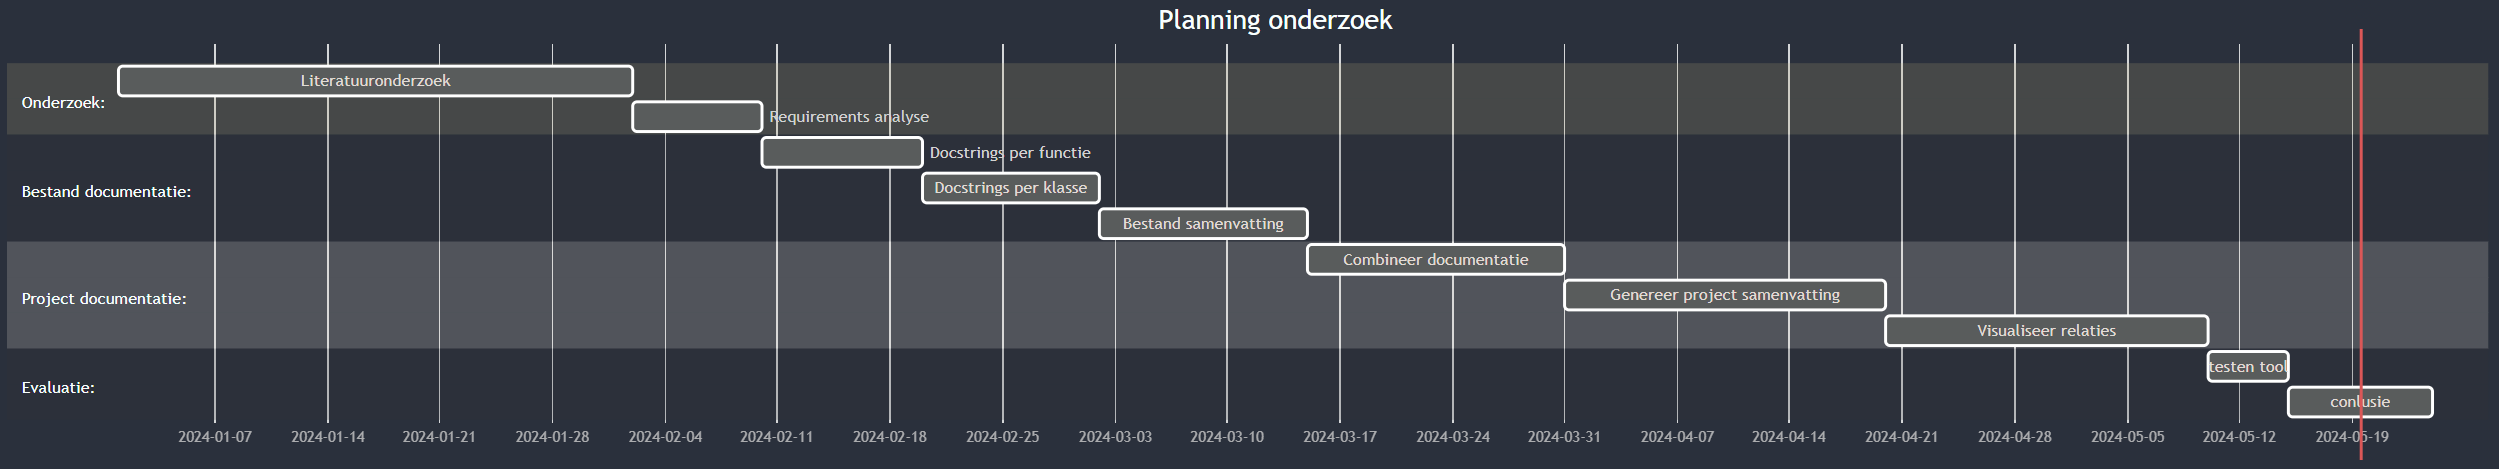
\includegraphics[width=1\textwidth]{flowchart.png}
    \caption{Tijdslijn onderzoek}
    \label{fig:flowchart}
\end{figure}

Het onderzoek is in drie fases opgedeeld. De eerste fase omvat de literatuurstudie.
In deze literatuurstudie wordt er onderzocht wat de huidige stand van zaken is omtent de technologie en mogelijkheden voor de documentatie van Python projecten met behulp van Large Language Modellen.
Zo wordt er gekeken naar wat LLM's zijn, hoe ze werken en wat bestaande tools zijn voor het genereren van documentatie.

Nadat er een duidelijk beeld gevormd is in de literatuurstudie, kan er begonnen worden aan de tweede fase.
Hier wordt er een tool ontwikkeld die een Python bestand kan analyseren en op basis daarvan documentatie kan genereren, aan de hand van het toevoegen van docstrings aan de code.
Dit doet het eerst per functie dan per klasse en uiteindelijk voor het gehele bestand. Dit kan later gebruikt worden om een samenvatting van het project te genereren in de volgende fase.
De uitkomst van deze fase is een tool die de documentatie van een Python bestand kan genereren. 
Door aan prompt engineering te doen, met het prompt dat meegegeven wordt aan de LLM, kunnen de bekomen docstrings accurater worden.
Verder wordt er gekeken naar hoe de documentatie van Python functies gebruikt kan worden voor het maken van een gehele samenvatting van het project.
Dit wordt gedaan op basis van huidige methoden om docstrings aan te maken en te gebruiken. 
Erna kunnen de verschillende docstrings met de bijhorende naam van de functie of klasse gebruikt worden om een samenvatting te genereren.
Deze informatie kan dan gegeven worden aan de Large Language Modellen om een samenvatting te genereren.

De derde fase beslaagt het documenteren van een geheel project.
Door de vorige fases te combineren, het documenteren van de individuele bestanden en het genereren van een samenvatting van het project, kan er een tool gemaakt worden die de documentatie van een geheel project kan genereren.
Deze documentatie bestaat uit de individuele documentatie van de bestanden en een samenvatting van het gehele project. 
Alsook wordt er gekeken naar hoe de relaties tussen de verschillende bestanden gevisualiseerd kunnen worden.

De laatste fase is het evalueren van de tool.
Hier wordt er gekeken naar de kwaliteit van de documentatie die de tool genereert.
Dit wordt gedaan door de documentatie van de tool te vergelijken met de handgeschreven documentatie van een project.
Dit wordt gedaan voor een bestand, een klein project en een groot project.

\section{Requirementsanalyse}
\label{sec:requirements-analyse}
De requirementsanalyse is een belangrijk onderdeel van het onderzoek. 
Hier wordt er gekeken naar wat de tool moet kunnen en wat de verwachtingen zijn van de tool.

\subsection{Functionele requirements}
\label{sec:functionele-requirements}
\subsubsection{Should Have:}
\begin{itemize}
    \item De tool moet in staat zijn om docstrings te genereren voor functies en klassen voor een Python bestand.\\
    De tool genereert docstrings voor functies en klassen in een Python bestand. Dit gebeurt door de code te analyseren en op basis daarvan een docstring te genereren.
    \item De tool moet in staat zijn om een samenvatting van een Python bestand te genereren.\\
    De tool maakt een samenvatting van een Python bestand. In deze samenvatting zitten de belangrijkste zaken van het bestand.
    Zijnde de functies en klassen die erin voorkomen en wat deze doen, alsook hun eventuele parameters en de uitkomst.
    \item De tool moet in staat zijn om een samenhangende samenvatting van een Python project te genereren.\\
    De tool dient een samenvatting te maken van een Python project. Deze samenvatting bestaat uit de individuele samenvattingen van de bestanden en een overkoepelende samenvatting van het project.
    Hierin staan alle functies en klassen die in het project voorkomen en wat deze doen, alsook hun eventuele parameters en de uitkomst.
    \item De tool moet in staat zijn om de relaties tussen de verschillende bestanden van een project te visualiseren.\\
    De tool visualiseert de relaties tussen de verschillende bestanden van een project. Zo is er geweten waar de bestanden naar verwijzen en van waar ze refereren.
\end{itemize}

\subsubsection{Could Have:}
\begin{itemize}
    \item De tool moet in staat zijn om de documentatie van een Python bestand te genereren in verschillende formaten.\\
    De tool genereert de documentatie van een Python bestand in verschillende formaten. Zo kan de gebruiker kiezen in welk formaat hij de documentatie wil.
    \item De tool moet in staat zijn om de relaties tussen de verschillende functies en klassen van een bestand te visualiseren op project niveau\\
    De tool visualiseert de relaties tussen de verschillende functies en klassen van een bestand op project niveau. Zo is er geweten waar de functies en klassen naar verwijzen en van waar ze refereren.
\end{itemize}

\subsubsection{Nice to Have:}
\begin{itemize}
    \item De tool moet in staat zijn om de documentatie van een Python bestand te genereren in verschillende talen.\\
    De tool genereert de documentatie van een Python bestand in verschillende talen. Zo kan de gebruiker kiezen in welke taal hij de documentatie wil.
    \item De tool moet in staat zijn om de documentatie van een Python bestand te genereren in verschillende stijlen.\\
    De tool genereert de documentatie van een Python bestand in verschillende stijlen. Zo kan de gebruiker kiezen in welke stijl hij de documentatie wil.
\end{itemize}

\subsection{Niet-functionele requirements}
\label{sec:niet-functionele-requirements}
\begin{itemize}
    \item De tool moet gebruiksvriendelijk zijn.\\
    De tool moet eenvoudig te gebruiken zijn. Dit betekent dat de tool intuïtief moet zijn en dat de gebruiker geen moeite moet doen om de tool te gebruiken.
    \item De tool moet betaalbaar zijn.\\
    Dit wil zeggen dat de tool geen hoge kosten met zich meebrengt.
    \item De tool moet snel werken.\\
    De tool moet snel werken. Dit betekent dat de tool snel de documentatie moet kunnen genereren. Sneller dan dat een persoon dit zou kunnen.
    \item De tool moet leesbare documentatie genereren.\\
    De documentatie die de tool genereert moet leesbaar zijn. Dit wil zeggen dat de documentatie duidelijk moet zijn en dat de gebruiker er gemakkelijk informatie uit kan halen.    
\end{itemize}

\section{Opstellen van een long-list tools}
\label{sec:long-list}
De long-list bestaat uit de verschillende tools die gebruikt kunnen worden voor het genereren van documentatie voor Pythonprojecten.
Deze tools worden onderzocht en vergeleken om te kijken welke het beste past bij de requirements van de tool.

De oplijsting van de tools is gebaseerd op de literatuurstudie en bestaat uit de volgende tools:
\begin{itemize}
\item Sphinx \autocite{Sphinx2023}\\
Een tool die gebruikt wordt voor het genereren van documentatie voor projecten met reeds een docstring. 
\item Doxygen \autocite{Doxygen2023}\\
Een tool die gebruikt wordt voor het genereren van documentatie voor projecten met reeds een docstring.
\item Pdoc \autocite{GallantHils2023}\\
Een tool die een API genereert voor Python projecten met reeds een docstring.
\item GPT4Docstrings \autocite{Trofficus2023}\\
Een tool die docstrings genereert voor Python projecten met behulp van GPT4 \textcite{OpenAI2023}.
\end{itemize}

Door de verschillende tools te onderzoeken en te vergelijken aan de hand van de requirementsanalyse kan er een keuze gemaakt worden welke tool het beste past bij de requirements van de tool.
Als er geen tool is die voldoet aan de requirements, kan er gekeken worden naar het combineren van verschillende tools of gebruiken van delen van verschillende tools om zo een eigen tool te maken.

Door eerst te kijken naar de programmeerttalen waarvoor de tools gebruikt kunnen worden, kan er al een eerste selectie gemaakt worden uit tabel \ref{table:vgl-tools}.
Zo kan er gekeken worden naar de tools die gebruikt kunnen worden voor Python projecten.
Vervolgens kan er gekeken worden naar het type documentatie dat de tools genereren.
Hierbij kan er gekeken worden naar de tools die docstrings genereren, aangezien dit de basis is voor het genereren van de gewenste documentatie.

\begin{table}[h!]
\centering
\resizebox{\textwidth}{!}{
\begin{tabular}{|c|c|c|c|c|}
\hline
Tool & docstrings & samenvatting bestand & samenvatting project & visualisatie \\ [0.5ex]
\hline
Doxygen & nee & ja & ja & ja \\
\hline
Sphinx & nee & ja & ja & nee \\
\hline
GPT4Docstrings & ja & nee & nee & nee \\
\hline
Pdoc & nee & ja & nee & nee \\
\hline
\end{tabular}}
\caption{Requirementsanalyse van de verschillende tools}
\label{table:ra-tools}
\end{table}

Uit deze tabel \ref{table:ra-tools} kan er geconcludeerd worden dat geen enkele tool voldoet aan de volledige requirements van de tool.
Doordat de Doxygen en Sphinx tools geen docstrings genereren en dit de basis is voor de documentatie, kunnen deze tools niet gebruikt worden.
Pdoc genereert enkel samenvattingen van een bestand dat reeds aangevuld is met docstrings en kan dus ook niet gebruikt worden.
Omdat GPT4Docstrings enkel docstrings genereert en geen samenvattingen van bestanden of projecten, kan er gekeken worden hoe deze tool dit doet.